\documentclass{article}
\title{\textbf{How to connect to AWS GUI using SSH tunneling}}
\author{}
\date{} 

\UseRawInputEncoding
\usepackage{graphicx}
% Links
\usepackage{hyperref}
\hypersetup{
    colorlinks=true,
    linkcolor=blue,
    filecolor=magenta,      
    urlcolor=cyan,
}
 
\urlstyle{same}

% Code Coloring
\usepackage{xcolor}
\usepackage{listings}
\lstset{
  language=bash,
  basicstyle=\small\sffamily,
  showstringspaces=false
  %numbers=left,
  %numberstyle=\tiny,
  numbersep=3pt,
  %linewidth=13cm,
  frame=tb,
  columns=fullflexible,
  backgroundcolor=\color{yellow!20},
  linewidth=0.9\linewidth,
  xleftmargin=0.1\linewidth
}

% Links
\usepackage{hyperref}
\hypersetup{
    colorlinks=true,
    linkcolor=blue,
    filecolor=magenta,      
    urlcolor=cyan,
}
 
\urlstyle{same}

% Code Coloring
\usepackage{listings}
\usepackage{color}
\usepackage{hyperref}

\definecolor{dkgreen}{rgb}{0,0.6,0}
\definecolor{gray}{rgb}{0.5,0.5,0.5}
\definecolor{mauve}{rgb}{0.58,0,0.82}
\lstset{frame=tb,
  language=C++,
  aboveskip=3mm,
  belowskip=3mm,
  showstringspaces=false,
  columns=flexible,
  basicstyle={\small\ttfamily},
  numbers=none,
  numberstyle=\tiny\color{gray},
  keywordstyle=\color{blue},
  commentstyle=\color{dkgreen},
  stringstyle=\color{mauve},
  breaklines=true,
  breakatwhitespace=true,
  tabsize=3
}

\begin{document}
\maketitle

\section{What is SSH ?}

\section{Linux sshd daemon ?}
\subsection{checking the status of the sshd}
\subsection{controlling the behavior of the sshd on the server}
In /etc/ssh, there are some configuration files which change the behavior of the server and the client as well
\begin{itemize}
  \item ssh\_config file is affecting the client.
  \item sshd\_config file is affecting the server.
\end{itemize}

\begin{center}
  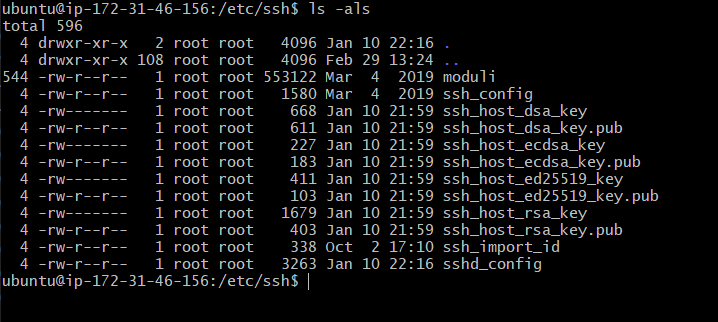
\includegraphics[scale=0.75]{resources/ssh/img/ssh-configfile.PNG}
\end{center}

let's speak about the sshd configuration file, and some of its configuration.
\begin{itemize}
  \item 
\end{itemize}

\subsection{passwordless login}
\begin{enumerate}
  \item Create a new key-pair
  \lstinputlisting[caption=Generate a new pair]{resources/ssh/basic/passwordless/1-ssh-keygen-client}

  \item Copy the public key to the server using \textit{scp}
  \lstinputlisting[caption=exchange the public key with the server]{resources/ssh/basic/passwordless/2-copy-to-server}

  \item append the new public key to the \textbf{~/.ssh/authorized\_keys} file
  \lstinputlisting[caption=Append it as authorized key]{resources/ssh/basic/passwordless/3-append-key}

  \item You can copy and append the keys in steps 2, and 3 directly using \textit{ssh-copy-id} command
  
  You will give it the private-key, and it will login the fist time and automatically append the authorized\_keys file for you. 
  \lstinputlisting[caption=Configure the sshd]{resources/ssh/basic/passwordless/3-1-use-ssh-copy-id}


  \item edit the \textit{sshd\_config} file to the the new key, and restart the sshd daemon to apply the new configuration
  \lstinputlisting[caption=Configure the sshd]{resources/ssh/basic/passwordless/4-edit-sshd-config}
  
  Here, you need to comment the \textit{PasswordAuthentication yes}, and un-comment the \textit{PubkeyAuthentication yes}.
  \begin{center}
    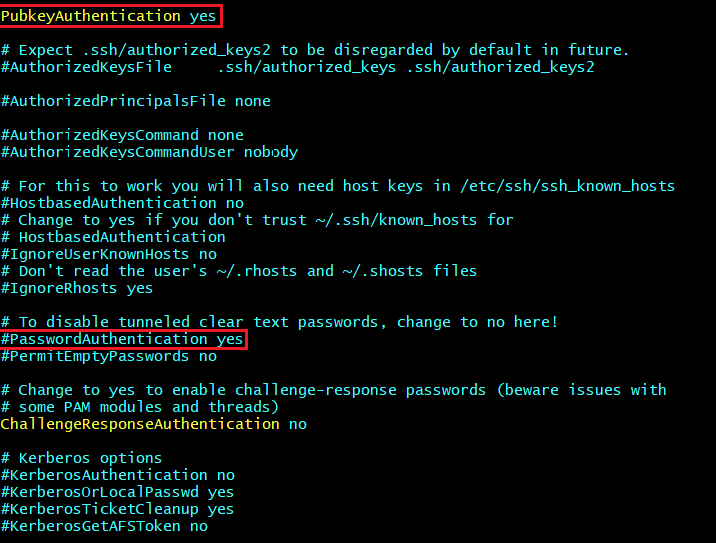
\includegraphics[scale=0.75]{resources/ssh/img/sshd_config.PNG}
  \end{center}

  \item communicate to the server using your private key
  \lstinputlisting[caption=Start a new communication]{resources/ssh/basic/passwordless/5-communicate-via-client}

  Note: you need to make sure the following permissions on the following client-side
  .ssh is given at least 700, and private-key file is given 600 

\end{enumerate}


\subsection{ssh-tunnels}

\begin{enumerate}
  \item Create your own AWS EC2 Linux Image (You can have a free tier)
  \item  Connect to your instance using SSH, You can use putty or any SSH client
  \item 
\end{enumerate}

\href{https://www.youtube.com/watch?v=6x_okhl_CF4}{Youtube video}

\section{Working with text processing using grep, sed and awk}
grep gnu regular expression parser
sed Stream editor
awk 

\end{document}